\documentclass{beamer}

\mode<presentation> {
\usetheme{Madrid}
\setbeamertemplate{footline}[page number]
\setbeamertemplate{navigation symbols}{}
}

\usepackage{graphicx}
\usepackage{booktabs}
\usepackage[short]{optidef}
\usepackage{tkz-graph}
\GraphInit[vstyle = Shade]
\tikzset{
  LabelStyle/.style = { rectangle, rounded corners, draw,
                        minimum width = 2em, fill = yellow!50,
                        text = red, font = \bfseries },
  VertexStyle/.append style = { inner sep=5pt,
                                font = \normalsize\bfseries},
  EdgeStyle/.append style = {->, bend left} }
\usetikzlibrary {positioning}
\definecolor{processblue}{cmyk}{0.96,0,0,0}
\definecolor{lightgray}{gray}{0.95}


\title[DNN and MILP]{Deep neural networks and mixed integer linear optimization}
\author{Mateo Fischetti, Jason Jo}
\date{\today}

\begin{document}

\begin{frame}
\titlepage
\end{frame}

\begin{frame}
\frametitle{Table of Contents}
\tableofcontents
\end{frame}

\section{Introduction}
\begin{frame}{Overview}
  \begin{itemize}
  \item Deep Neural Networks (DNN) are composed of layers of neurons
  \item Each neuron calculates an affine combination of the outputs of the previous layer;
  \item Finally, each neuron applies a non-linear operator on the result and feeds it to the next layer
    \begin{itemize}
    \item A common operator is the ReLU function
    \end{itemize}
  \end{itemize}
\end{frame}

\section{Definitions}
\begin{frame}{Definitions}
  \begin{itemize}
  \item A DNN is composed of $K+1$ layers, numbered $0$ to $K$
    \begin{itemize}
    \item Layer $0$ is a ``fake'' layer, and consists of the input of the network
    \item Layer $N$ is the output of the network
    \end{itemize}
  \item Each layer $k$ is composed of $n_k$ neurons (or units), numbered from $1$ to $n_k$
  \end{itemize}
\end{frame}

\begin{frame}{Definitions}
  \begin{itemize}
  \item Let $x_k \in \mathbb{R}^{n_k}$ be the output vector of layer $k$, and $x^j_k$ is the scalar output of \texttt{UNIT}$(j,k)$
  \item For each layer $k \geq 1$, \texttt{UNIT}$(j,k)$ computes its output vector using the following formula:
  \end{itemize}
  $$
  x^k = \sigma(W^{k-1} x^{k-1} + b^{k-1})
  $$
  \begin{itemize}
  \item where $\sigma(.)$ is a non-linear function, $W^{k-1}$ and $b^{k-1}$ are a matrix of weights and a vector of activation biases
    \begin{itemize}
    \item One possible operator is the ReLU~(rectified linear unit) function
    \end{itemize}
  \end{itemize}
\end{frame}

\begin{frame}{Proposal}
  \begin{itemize}
  \item Use $W^k$ and $b^k$, $\forall k \in [0, K]$ to build an optimization model
    \begin{itemize}
    \item Applications in adversarial examples generation and activation visualization
    \end{itemize}
  \end{itemize}
  \pause
  \begin{block}{Problem}
    \centering
    $\sigma(.)$ is not linear
  \end{block}
\end{frame}

\begin{frame}{ReLU Operator}
  $$ \sigma(x) = \text{ReLU}(x) = \text{max}(0, x) $$
  \pause
  \begin{figure}[H]
    \centering
    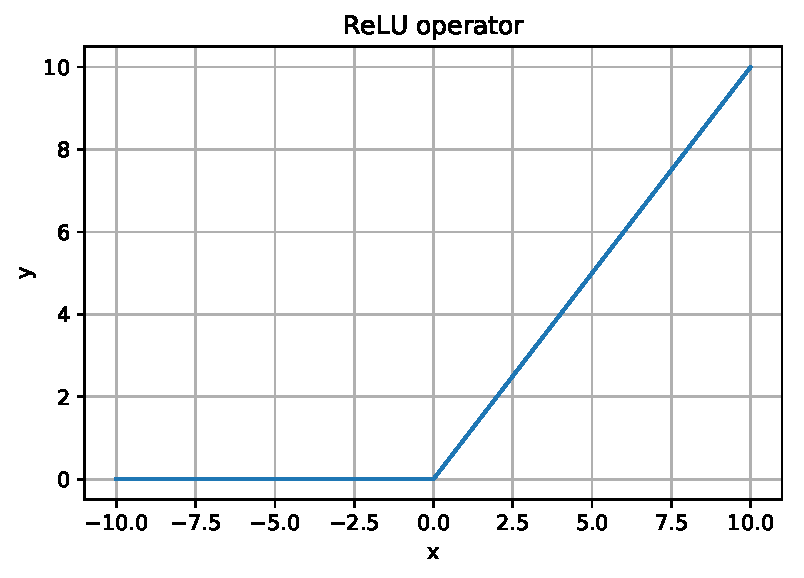
\includegraphics[width=0.8\columnwidth]{relu}
  \end{figure}
\end{frame}

\begin{frame}{Model}
  \begin{mini!}
  {x,y}{\sum_{k=0}^K \sum_{j=1}^{n_k} c_j^k x_j^k  + \displaystyle \sum_{k=1}^K \sum_{j=1}^{n_k} \gamma_j^k z_j^k}{}{}
  \addConstraint{\sum_{i=1}^{n_{k-1}} w_{ij}^{k-1} x_i^{k-1} + b_j^{k-1}}{= x_k^j - s_j^k \label{relu-1}}
  \addConstraint{x_j^k, s_j^k}{\geq 0 \label{relu-2}}
  \addConstraint{z_j^k}{\in \{0,1\} \label{relu-3}}
  \addConstraint{z_j^k = 1 \rightarrow x_j^k}{\leq 0 \label{relu-4}}
  \addConstraint{z_j^k = 0 \rightarrow s_j^k}{\leq 0 \label{relu-5}}
  \addConstraint{lb_j^0 \leq x_j^0}{\leq ub_j^0}{, j = 1, \dots, n_0 \label{limits-xn0}}
  \addConstraint{lb_j^k \leq x_j^k}{\leq ub_j^k \label{limits-xnk}}
  \addConstraint{\overline{lb}_j^k \leq s_j^k}{\leq \overline{ub}_j^k \label{limits-sn0}}
  \end{mini!}
\end{frame}

\begin{frame}{Model}
  \begin{itemize}
  \item All weights $w_{ij}^{k-1}$ and biases $b_j^{k-1}$ are calculated at the training stage
  \item The objective function costs $c_j^k$ and $\gamma_j^k$ are defined according to the problem
  \item Conditions~\ref{relu-1},~\ref{relu-2},~\ref{relu-3},~\ref{relu-4}, and~\ref{relu-5} define the ReLU output for each neuron
  \item Conditions~\ref{limits-xn0},~\ref{limits-xnk}, and~\ref{limits-snk} are known upper and lower bounds for $x$ and $s$
  \end{itemize}
\end{frame}

\begin{frame}{Model discussion}
  \begin{itemize}
  \item BLA
  \end{itemize}
\end{frame}

\section{Applications}
\begin{frame}
  \begin{itemize}
  \item This model is unsuitable for training $\rightarrow$ leads to overfitting
  \end{itemize}
\end{frame}

\begin{frame}
  \Huge{\centerline{Fin}}
\end{frame}

\end{document}